\documentclass[11pt, letterpaper]{article}
\title{Push: a DISC shell}
\author{Noah Evans\\
IBM Research\\
Nara Institute of Science and Technology\\
noah-e@is.naist.jp\\\\
Eric Van Hensbergen\\
IBM Research\\
ericvh@us.ibm.com\\
}
\usepackage{fullpage}
\usepackage{graphicx}
\date{}
\begin{document}
\maketitle
\pagebreak
%\begin{abstract}
%
%Pipes were a huge advance in software engineering, allowing the
%composibility of previously isolated programs regardless of programming
%language. With the move to Data Intensive Supercomputing there is
%a similar trend towards the use of pipelines. Systems define graphs
%of processes, the edges of the graphs representing pipes and their
%vertices represent computation on a system. With these systems and
%a new class of languages built on top of them researchers can solve
%"pleasantly parallel" problems more quickly without worrying about
%explicit concurrency.
%
%This approach is powerful and appropriate for many problem types.
%However as of yet none of these systems have been able to recapture
%the conceptual simplicity and ease of use of Unix pipelines as
%implemented by the shell. We have implemented a shell using DISC
%principles, PUSH, which contains built in operators to provision
%and connect virtual and/or physical OS instances  Process
%interconnections are composed using synthetic file systems, pushing
%the distributed complexity into the operating system and out of
%middleware.  In this paper we explore the motivations, design and
%implementation of the PUSH shell showing how it can be used to solve
%many DISC problems. Finally we show how the system can be used with
%two current utility computing systems, IBM's kittyhawk and Amazon's
%EC2 to transparently interconnect and run DISC processes using only
%the terseness and expressivity of the shell.  Introduction As Data
%Intensive SuperComputing(DISC) becomes increasingly mainstream there
%have been a proliferation of different languages allowing the
%provisioning, filtering, distribution and aggregation petabytes of
%information over a variety of systems. However with this great there
%is nothing like the terseness and simplicity of the simple unix
%'sort | uniq -c'. Most are still in programming languages and many
%of them ape unix's model of pipelines.
%\end{abstract}
\section{Introduction}

With the advent of huge publicly available data sets such as sensor networks, online transactions, and web data, users are now able to work with much more data than ever before. However it is also impossible to deal these data sets in a reasonable amount time and economically even using the most powerful isolated machines. This problem is described in depth in (original map reduce).  

Data Intensive Scalable Computing(DISC)[cite] has become a standard tool to solve research problems using these datasets. By dividing the data into structured data and then distributing that data onto large sets of individual computational resources it becomes possible to solve previously intractable problems using large clusters of commodity hardware. Correspondingly there has been a proliferation of different languages and systems allowing the provisioning, filtering, distribution and aggregation of petabytes of information over a variety of systems.  

At the lowest level there are systems like Google's MapReduce(cite), Microsoft's Dryad and Apache/Yahoo's Hadoop which provide a job scheduler, work partitioning and execution. Built on top of these systems are languages like Sawzall, DryadLinq and Pig Latin which allow the expression of DISC jobs and workflows without the bookkeeping and verbosity of manipulating DISC systems directly.    
\begin{figure}[htp]
\centering
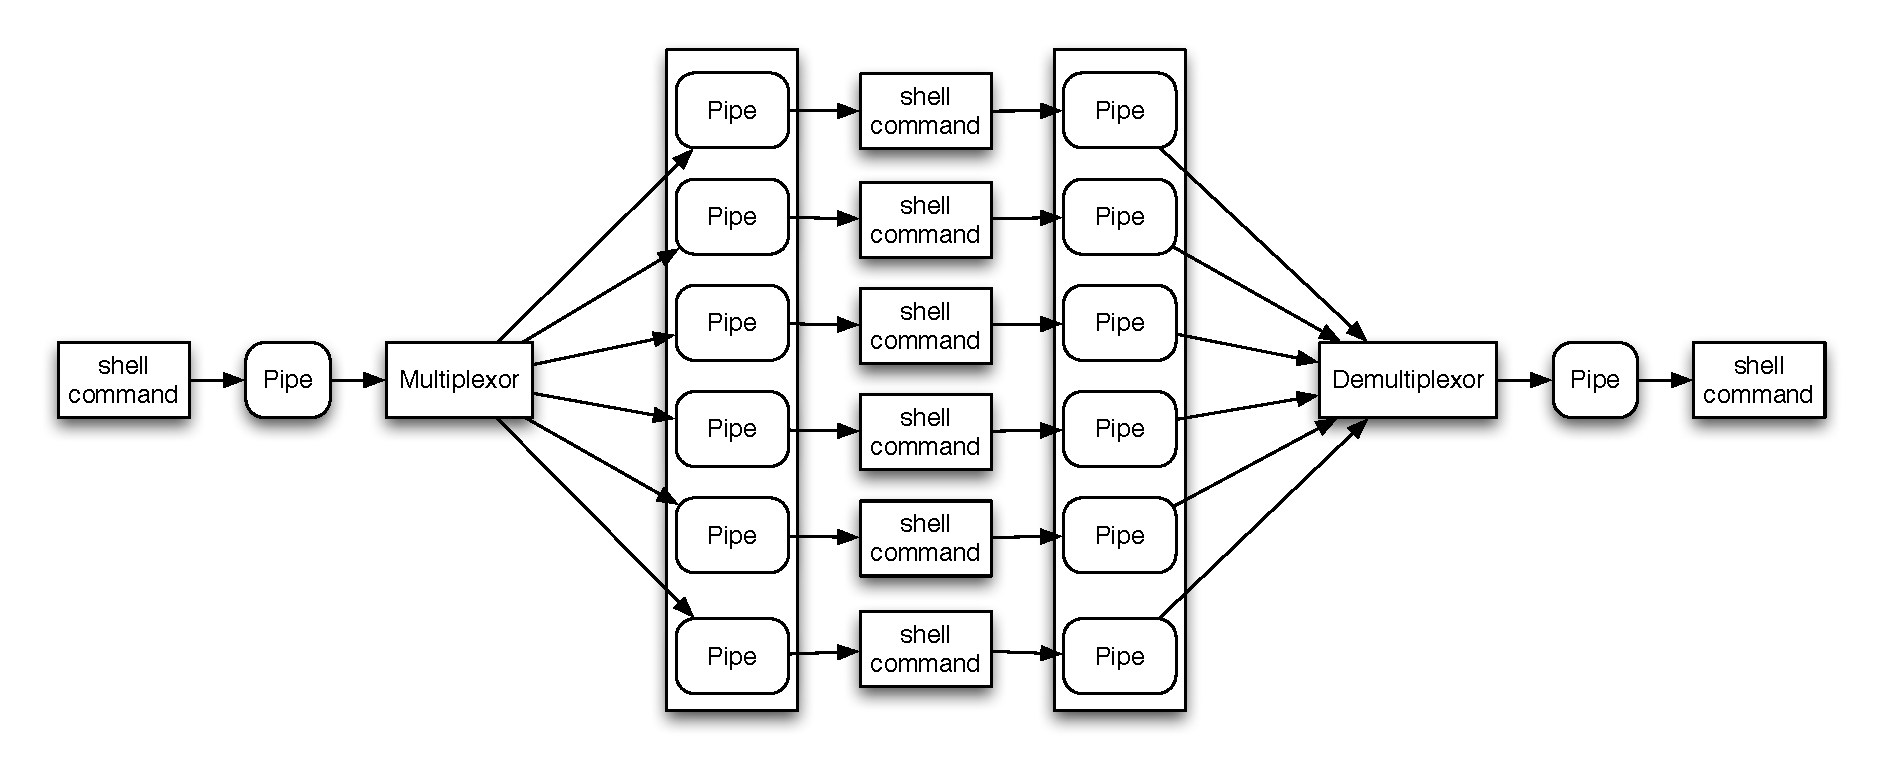
\includegraphics[width=4.5in]{pipestruct.eps}
\caption{Pipe structure}\label{fig:pipestruct} 
\end{figure}
More specifically DISC systems provide a two level hierachy to solve problems. Users can use DISC languages to create DISC workflows but these workflows are tied to the systems that they are written on. This makes solutions written for one DISC system inherently incompatible with other DISC systems. It also ties the solutions to a particular platform in this case, middleware, workflow and language.   

\renewcommand{\topfraction}{0.85}
\renewcommand{\textfraction}{0.1}
\begin{figure}[htp]
\centering
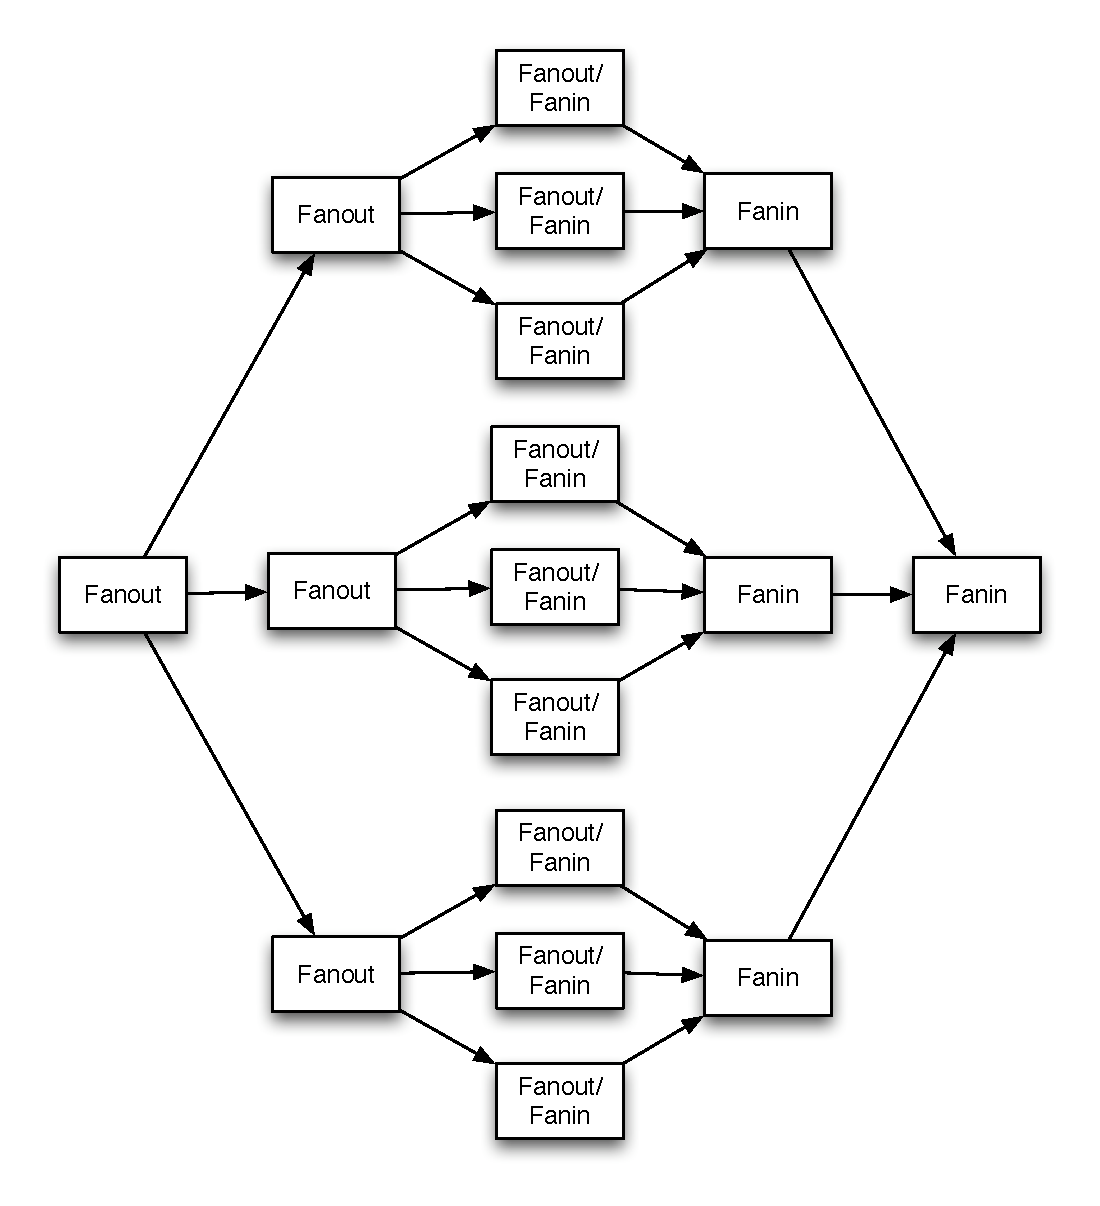
\includegraphics[height=2.5in]{fofigraph.eps}
\caption{Transverse momentum distributions}\label{fig:fofigraph}
\end{figure}
\begin{figure}[htp]
\centering
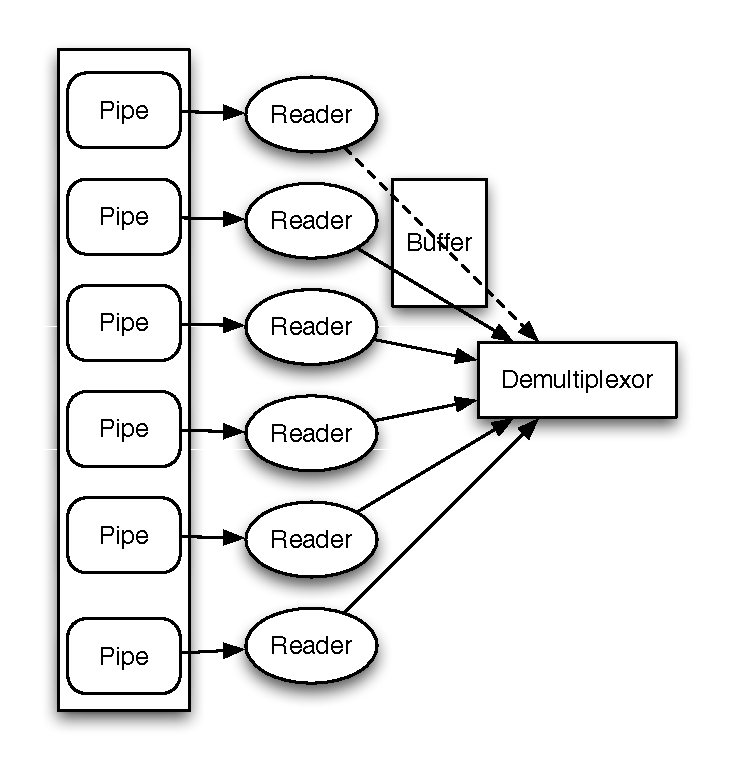
\includegraphics[height=2.0in]{demux.eps}
\caption{Transverse momentum distributions}\label{fig:demux}
\end{figure}
\begin{figure}[htp]
\centering
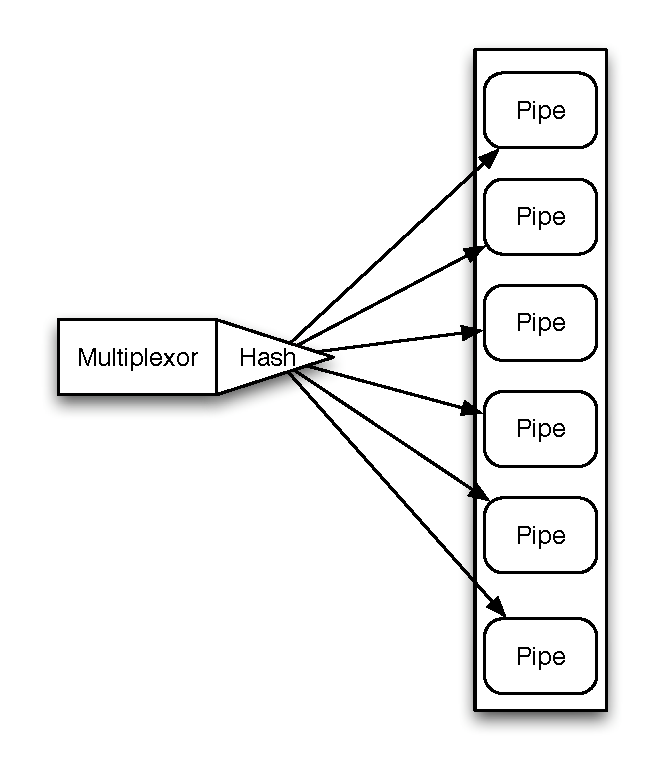
\includegraphics[width=2.0in]{mux.eps}
\caption{Multiplexor}\label{fig:mux}
\end{figure}
These languages provide automated control flow and pipelines, but none of these languages match the terseness and simplicity of the UNIX shell model (e.g. 'sort | uniq -c') which can compose a number of smaller programs into a coherent workflow to solve more complicated problems quickly. 

Unix got this flexibility of workflow creation by using a three level hierarchy. At the lowest level Unix provided a set of standard system calls that worked the same between systems. Some of these calls instantiated computation like fork() and allowed device independent io through file descriptors, system level io handles which standardized the communication between programs and devices.  

compiled programs could then use these standard calls which worked the same way between systems to allow the portability between systems, as long as you followed the unix interface you programs could be compiled for any unix system(as long as you kept other issues in mind like endianess).   

In addition by standardizing upon certain io ports, standard input, output and error programs could be composed with one another through pipelines, which rerouted a program's output descriptor into the input descriptor of another, allowing programs to work together in streams *with no explict knowledge of this chaining built into the program itself*.   

Contrast this with the current way of writing solutions for DISC systems which use vastly different problem solving architectures and methods in the system. To port tools from one DISC system to another users must to completely reimplement tools, quite often with a different philosophy and data model to get what they want. Many research groups, notably microsoft's dryad system(cite) have noticed the discrepency and have attempt to make it possible to use preexisting sequential code to solve problems.[cite]  

figure {
manipulation layers
}

figure {

}
However the tools they provide are still cumbersome. Dryad's workflow creation program requires the user to manually specify and manipulate graphs of executable programs, "vertices" with and their connections "edges" to create and execute programs. A user has to meticulously plan and implement the distribution of their computation.   


Compare this process to the traditional writing of a unix shell script. Users use a vocabulary of components, scripts, executables and shell commands, which users can invoke quickly and then iteratively refine the resulting workflow until a desirable solution is reached.

However the Dryad approach is appropriate to the current context of DISC program writing, where the systems used are extremely large, expensive and set preexisting special purpose computation resources shared between many users. The cost of CPU time makes programmer time less important, ad hoc iterative solutions are a waste of system and resource time. [cite Sawzall paper for backup] 

However with the advent of systems like EC2[cite], individuals can create ad hoc DISC systems without the same massive overheads that traditionally kept DISC systems the domain of companies with large resources like Google and Microsoft. An EC2 user can create 320 instances for an hour of processing for \$32. Google spends XXX TD on infrastructure. A user can run DISC jobs easily at a fraction of the cost. the same job XXX TD costs XXX TD when instantiated on EC2.

In addition to the advantages of being able to create your own DISC systems using EC2, by being able to use an ad hoc virtualized environment there are many instances where having a heavily optimized the complexity and power of an optimized DISC system is unnecessary. 

If a user has a well defined plan for implementing a solution to a DISC problem then the user would be better served by using a DISC language, but for many tasks a user may want to distribute a large amount of data and computation to a variety of nodes without the overhead necessary to a DISC system. Currently users can do much of this distribution manually with a sequence of remote execution commands like ssh(1) but this process is cumbersome and difficult as well as losing much of the original context of the originating system's environment, file system and control flow.

So now users are at an impasse. They can deploy huge DISC systems that work within certain domain and company specific languages or use cumbersome approaches are difficult to deploy for ad hoc DISC solutions. There are systems like Hadoop[cite] which attempt to be an open platform to solve user tasks but they are currently limited to map/reduce type problems, not the more flexible "vertices" and "channel" metaphor of Dryad.

(Doesn't fit with current flow)

With the ready availability of cheap, easy to provision cluster resources, we feel the time is ripe for the development of a more generalized framework for DISC that leverages the dynamic availability of resources, facilitates the use of any language or runtime, and has the simple, terse, composability of the UNIX shell. Specifically we want to create a system that dynamically provisions computation and then interconnects it automatically while still being language independent and retaining a common context between systems.
  

We argue that this kind of solution is better implemented at the systems rather than the middleware level. By implementing DISC systems at the system level you provide a standard set of resources that allow the user to build DISC applications in a language and middleware independent manner. 

\section{Overview}
We observe that many DISC middleware's capabilities  are designed to solve problems that were previously handled at the systems level. Middleware     creates a higher level distributed workflow system *on top* of the system it is running on. 

At the systems level we need to solve two main problems:

First we need a way to dynamically provision computation easily and portably. One of the reasons for Unix's longevity and power is a set of simple abstractions that map across hardware platforms, fork, exec etc... may have very different internals on different machines but to the compiled software they work exactly the same. Currently outside of a few systems(snowflock) data provisioning implemented incompatably within each type of middleware.    

Second, dynamically provisioned systems don't have a common way of partitioning, allocating and working a new instance. Amazon's EC2 and IBM's kittyhawk both dynamically partition nodes, but they each have a differing interfaces which makes writing portable programs based on provisioning data difficult. 
 
 

Based on these two observations we have created a scalable, portable DISC shell, Push, using calls for dynamic provisioning and a pipe abstraction which makes it possible to do many to one and one to many communication. 

One of the principle advantages of the unix shells is that they allow the composition of a lot of different tools(which themselves took a lot of work to create and establish) with a simple language which doesn't take much time to write(or work to establish). With a bit of creativity a proficient unix user can come up with quite complex workflows to solve problems much more quickly than if they had implemented the entire solution in a lower level language(e.g. C or Perl). 

However moving to a DISC pattern from the traditional shell model of linear pipelines over bytestreams is nontrivial. 
As [sawzall] notes you need to be able to cleanly separate input streams into records and then show that they can dealt with in a commutative(need more familiarity with this) way. By separating input and output into discrete unordered records they can be easily distributed and coalesced.

The traditional Unix way of composing programs is unsuited to this strategy, currently when unix programs communicate through pipes they write using buffered byte streams which have no concept of the structure of the underlying data flow. Since unix programs write data according to buffer boundaries instead of record boundaries any attempts to distribute buffered data unmodified from a pipe will fail---output will not respect record boundaries. This failure to separate data boundaries cleanly leads to situations where the distributed output is meaningless, for example failing to respect xml element boundaries or newlines in line based records. 
   


We solve this problem by changing the semantics of pipes  we add an intermediary process in between pipe instantiations which mediates output from one set of writing processes to another set of reading processes.    Instead of a one to one streaming of buffers between processes the intermediate process between pipelines parses and separates data according to record boundaries. It then writes the parsed data to a specified reader. By using an intermediate process shell commands can be run unaltered, they still write buffered byte streams the shell itself takes care of the record separation and distribution. This separation preserves traditional program semantics while allowing the distribution of shell program output.

This process is referred to as fanning in and fanning out from the shell. 

(Talk about components here. )  
\section{An example}

To solve problems on large data sets users need to have the ability to take a huge number of files and  perform some form of transformation, aggregation and/or analysis on that data.  

A typical example from our particular experience(natural language processing) is to apply an analyzer to a huge set of files, a "corpus". Users go through each file, a list of sentences, one sentence per line and then tokenize the sentence into words, finding the part of speech and morphology of the words that make up the sentence.

This sort of task maps very well to the DISC model, we have a large number of discrete sets of data whose order is not necessarily important. We need to perform a computationally intensive task on each of the sentences, an operation on small, discrete records an ideal task for parallelization. 

Push was designed to exploit this mapping.   . For example, to get a histogram of the distribution of Japanese words from a set of documents using chasen, a Japanese morphological analyzer, we take a set of files in this case a XXX TD set of sentences and then distribute them to a cluster of machines on our network. The command is as follows:  
¥begin{verbatim}
example{
push -c '{ORS=./blm.dis; du -an files |< xargs os chasen | awk '{print \$1}' | sort | uniq -c >|  sort -rn
}
¥end{verbatim}
  
The first variable ORS declares our record multiplexor module, the intermediary used to ensure that the input and output to distributed pipes are correctly aligned to record boundaries. du -n gives a list of the files(note that our du is a bit different from the canonical Unix du, it replaces much of find's functionality) which are then "fanned out"(|<) using a combination of a ¥emph{multipipe}, an ordered set of pipes, and a \emph{multiplexor} which determines which pipes are the targets of each unit of output.  This fanned out data goes to xargs on other machines which then uses the filenames(sent from the intantiating machine) as arguments for chasen. The du acts as a command driver, fanning out file names to the individual worker machines. The workers then use the filenames are arguments to xargs. Using the output of the analyzer awk extracts the first line fields(Japanese words) which are then sorted and counted using uniq.  Finally these word counts are "fanned in"(>|) to the originating machine which then sorts them. The distribution mechanisms are described in detail in a later section.    

 
 

\subsection{Multiplexors and Multipipes}

Much of the interesting aspects of the system come from the interactions between pipes, multiplexors and multipipes.    


Multiplexor modules expose an interface(figure) which provides the ability to determine the desired record boundaries upon which to split the output data. The different modules are implemented as a set of filter requests asking for buffers of bytes. The shell provides these buffers by reading from a pipe attached to the standard output of the multiplexing program. Once these buffers have been provided the multiplexor module splits the data and then determines which of pipe of a multipipe to write to. The choice of which multipipe to target is left as a decision to the module. Different data formats may have different output requirements. For our main module, which operates on string values we use a djb2 hash[cite] to choose the target pipe and separate records on newline boundaries.

Demultiplexing from a multipipe is performed by creating a many to one communications channel within the shell. The shell creates a reader processes which connect to each pipe in the multipipe. When the data reaches an appropriate record boundary a buffer is passed from the reader to the shell which then writes each record buffer to the output pipeline. 

This description leaves out one important caveat, how does the shell handle data that overruns buffer boundaries? In our current implementation of a multiplexor module the multiple reading operation is done by keeping a table of buffers which match the number of pipes in a multipipe. In the event that a buffer overflow(i.e. a record is too large for the buffer) the buffer table coalesces buffers until a complete record is obtained. In the event of buffer underflow(i.e. there are leftovers after every record in the buffer is consumed) the system attempts keeps the leftover buffer and appends it to the start of the next one, ensuring record continuity. This behavior has an effect on performance which is mentioned in the Performance section. 

figure{
multiplexing and demultiplexing data. 
}

  

\section{Push language overview}

        

To implement push we extended an existing shell, mash(cite), from which we inherited a rich interpreted scripting language. Push functions much like traditional shell with the added goal of distributing computation over pipelines in order to make implementing DISC workflows easier.   

Push inherits its shell behavior from mash(1), it treats variables as lists of strings and has no native handling for anything other than strings. It has native regular expression support and it has a novel ability to do declarative shell programming through a make like syntax incorporated in the shell itself.

Push differs from traditional shells by native support for records over pipes. This facility is similar to the argument field separators, IFS and OFS, in traditional shells which use a pattern to determine how to tokenize arguments to control flow.   Push provides two variables ORS and IRS which are record separators. They work in a similar way to awk's RS specifying record boundaries, defining the separator between records that the system distributes or coalesces with multiplexors. This variable does not represent an expression but rather a module which defines the parser for the output and the distribution algorithm for their outputs. 

     Multiplexors can be instantiated by the use of two types of multi-pipes, a multiplexing fan-out(|<)  and a demultiplexing fan-in(syntax >|) which defines how to take multiple inputs and coalesce its records and one input and distribute its records respectively. This combination allows the machine to distribute to and from multiple simultaneous threads of control. The system defaults to separating records based on newlines, although an xml multiplexor is available and more will be available in the future.    
   

  

\subsection{Fanning in and Fanning out}

Push's novelty comes from its ability to create arbitrary graphs of distributed processes at the shell level. Users begin by fanning out some data which goes to the standard in of a bunch of processes and then goes to the standard in of a bunch of processes. ¥figure of graphs

So what a Push program normally does is take some initial data source, a list of filenames, a set of records in a file and then distributes input to a bunch of items in a file. when this data is distributed then the new program instances themselves have the ability to fan in and fan out arbitrary subgraphs as well. 

Since each fan out is matched to a fanin the graphs gradually coalesce until the output merges to the original instantiating pipeline. This process allows the user to create arbitrary graphs. 

The following examples better illustrates this process:

example{
cat |< cat |< cat |< cat >| cat |> cat >| cat }
}

Fanins and fanouts are grouped like parentheses. If the user wishes to choose a different structure for the grouping of a push invocation they can group the elements with brackets to change the distribution to a more desirable structure. 

The usual way for a user to write a push program is:


  

figure{

}caption{
the way things are provisioned in this process
}


\subsection{Execution Model}

  


Push functions much like a normal shell but multipipes and the fact that computation is potentially taking place on different machines can have quite different effects from what a user might expect. 


One major example is redirections. A redirection is similar to a pipe in that it redirects a file descriptor normally attached to the console to another file descriptor which may or may not refer to an actual file. 


The other example is file arguments. Because programs are not necessarily running on the same machine it is difficult. To fix this problem push takes advantage of Inferno's distributed file systems(where everything is a file) to create a standard environment between systems so that shell commands seem similar and that users can feel like they're executing on the same system image. The state is preserved throughout the machines. 

copies the namespace of the system(see [cite] for details of inferno namespace, think of namespaces as per process mount tables) allowing each push instance to see the same environment even when instantiated on remote machines. 

This provides another advantage, rather than having to stream files over multipipes users can actually send filenames over the pipe to remote systems which can then be used by commands like xargs which can then operate on the local files, better taking advantage of locality of data and limiting the congestion of the network streams caused by the multipipes. 

\section{Resource conservation and understanding distribution}

 

Push has a few features that are very different from traditional shells. 

One of these is the ability to allocate new operating system instances to use as a way of acquiring new computational resources. One of the central goals of push is to be able to scale up simple solutions to problems and its language features reflect this. 

Since Push scripts can potentially be very costly to run users can specify resource limits and perform test evaluations to make sure that their scripts will work as intended push has two flags '-d' and '-g' which aid in the debugging of the distribution of shell scripts.

-d provides the manual selection of resources. by choosing the d option users can figure out how many pipes and total machines they want to use. there is a special value '-1' implies that the user wants to use the maximum amount of resources avaiable. 

-g graphs the composition of a push script. It gives the user the ability to see how their script would run by generating a dot file representing the composition. -g implies the Enoexec flag, avoiding execution of the script. 

 
\section{Performance}

We also have a problem with IO. When you're reading and writing a pipe you're still writing a local thing on a local machine. Your within an XXX TD(how much faster are local, remote and programmatic pipes). The cost of reading and writing is XXX we talk more about these relative differences in the Evaluation section.   

Performance of Push programs can vary widely depending on the needs of the task to be performed. For IO bound tasks the construction of data flow by the user can be very important. For cpu bound tasks the problem. 

However to show the relative performance hit of instantiating the multiplexor and multipipes we wrote a benchmarking program that 
The shell works like a normal shell it spawns programs, putting them together with other programs. Where it differs is its ability to fan in and fanout program output according to a predefined set of multiplexer rules, which can differ between different parts of a multipipe. 

\subsection{Pipeline instantiation}

To test the effects of our multipipe infrastructure compared to a regular shell we wrote a shell script which explicitly dictates the size of the multipipes given to push and then instantiated a simple filter which passed its output unmodified through a pipe, with the goal of testing how long it takes to instantiate and use multipipes.

figure{
command XXX TD
}
table{
regular pipes
0.001l 0.009r 0.01t
2 pipes
0.002l 1.278r 1.28t
4 pipes
0.002l 1.239r 1.241t
8 pipes
0.001l 1.195r 1.196t
16 pipes
0l 1.146r 1.146t
32 pipes
0l 1.084r 1.084t
64 pipes
0.001l 1.077r 1.078t
128 pipes
0.001l 1.103r 1.104t
256 pipes
0.001l 1.032r 1.033t
512 pipes
0l 1.061r 1.061t
1024 pipes
0.001l 1.026r 1.027t
2048 pipes
pipe failed: no free file descriptors
could not find multipipe: no free file descriptors
2295 "Pushlib":fail: push system error
0.001l 0.293r 0.294t
}

The results of this are interesting, they show that the main bottleneck is the record handling in our pipe multiplexing. the more 
do it on the local network. 

\subsection{IO Bound tasks}

Next we tested data through put for a variety of tasks. showing how the data slowed down when tasks were sent over a variety of machines, then we explored how fast it went when only filenames of a standard system image were sent over the pipe. 


(TD)

\subsection{CPU bound tasks}

Finally one of the primary goals of Push is to allow cpu intensive tasks, bioinformatics and natural language processing tasks in particular, to be distributed over as many machines as possible to complete quickly. 

\section{Future Work}

Right now Push is good for creating ad hoc solutions to DISC problems. but it has issues with how programs are created and how they behave.

Many unix programs do not support writing to standard in and standard out. A good example is a file that requires two file arguments. This limits the efficacy of push. 

We need wider coverage of modules over different file formats. A way of passing arguments to multiplexor modules would also be very useful. For example a multiplexor xml module that supported Xpath(cite) could be very useful for extracting relevant chunks of data from an xml file and then post processing them with Unix tools. 

However many unix tools do not support a good DISC model of preserving locality when writing programs. One of the principle advantages of Google's approach to solving DISC problems is that they are careful to use the locality of the system. Push does not have any explicit methods for preserving locality.

However with care it's possible to use Push's approach to better preserve locality, sending file names rather than files etc... Inferno provides the ability to do distribute files easily but right now it does not have any support for caching files or using a distributed filesystem like Google's gfs(cite).

The ability to create distributed files could lead to a system where we could create distributed databases similar to Bigtable which would better preserve the locality of data. 

Another problem that push has is that while Push can support multiple distributed machines, its underlying operating system Inferno does not support multiple cores. The ability to support multiple cores in Inferno's OS would allow local distribution of tasks as well. Greatly increasing Push's efficiency. 

Finally it can cost a lot of money to use Push if you are using a system like Ec2. Naive users can conceivably unkowningly spend large amounts of money using an incorrect push invocation. Some way of setting limits to the amount of systems/resource time used by a push invocation would better allow push to protect users from mistakes. 
\section{Conclusion}

With the advent of a variety of utility computing systems users have the ability to create their own clusters of machines. However the ability to quickly and easily use these clusters doesn't exist yet. Users must use commands or preexisting middleware to create and solve problems. 

We presented Push a shell for DISC problems. Push reduces the complexity of instantiating, provisioning computation and output in a way that conforms to the traditional way unix users expect to deal with commands. This allows users to chain a variety of preexisting unix tools unmodified, combining compiled programs domain specific languages and shell scripts. 

This allows users to take advantage of their ability to create their own ad hoc DISC systems, static middleware based approaches. The idea is to allow users to incorporate their own stuff in a data independent way. 

Push gives users the ability to create solutions to ad hoc DISC problems quicker and more easily than traditional systems. By moving the responsibilities for distributing computation out of middleware and back to the system it becomes possible to compose traditional unix commands over a variety of machines. 

\section{Acknowledgements}
 
I would like to thank Sape Mullender and James Mckie from Bell Labs for giving me feedback and advice on the construction of Push. I wouBruce Ellis explained the original goals and design of mash.  I would also like to thank Jon Appavoo and Amos Waterland for helping me set up Kittyhawk and answering my questions. I would also like to thank Jordi Polo and William Polensky for proofreading help and paper organizing suggestions. Finally I would like to thank my advisor Masayuki Asahara for advice and support.  Part of the research for this paper took place under Government Contract \#
\cite{thompson1993hwo}
\bibliographystyle{plain}
\bibliography{thesis} 
\end{document}




